\documentclass{article}
\usepackage{pgfplots}
\pgfplotsset{compat=newest}

\begin{document}
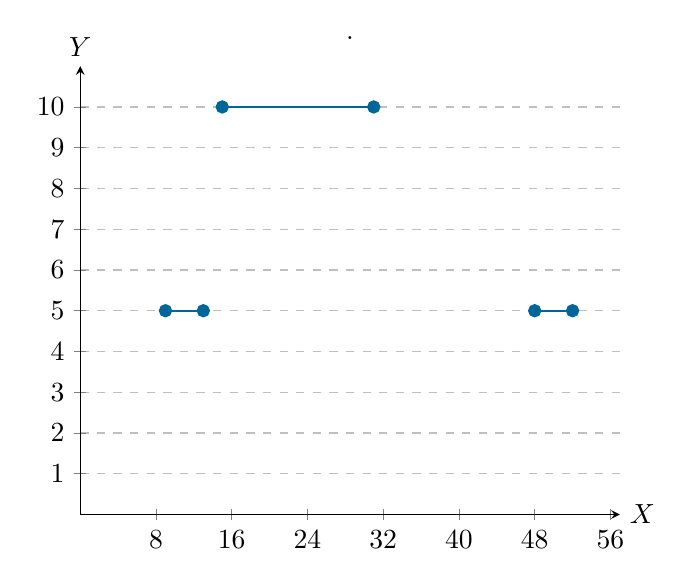
\begin{tikzpicture}
\begin{axis}[
    title={.},
    axis lines=middle,
    xlabel=$X$, xlabel style={at=(current axis.right of origin), anchor=west},
    ylabel=$Y$, ylabel style={at=(current axis.above origin), anchor=south},
    xmin=0, xmax=57,
    ymin=0, ymax=11,
    xtick={0,8,16,24,32,40,48,56},
    ytick={0,1,2,3,4,5,6,7,8,9,10},
    yticklabels={0,1,2,3,4,5,6,7,8,9,10},
    %legend pos=north west,
    ymajorgrids=true,
    grid style=dashed,
]
\addplot[color={rgb:red,0;green,2;blue,3},mark=*, thick, mark options={draw=none}] coordinates {
    (31,10)
    (15,10)
};
\addplot[color={rgb:red,0;green,2;blue,3},mark=*, thick, mark options={draw=none}] coordinates {
    (52,5)
    (48,5)
};
\addplot[color={rgb:red,0;green,2;blue,3},mark=*, thick, mark options={draw=none}] coordinates {
    (9,5)
    (13,5)
};
\end{axis}
\end{tikzpicture}
\end{document}
